% -------------------- DON'T EDIT ----------------------------------------
\documentclass[a4paper,12pt,oneside,openany]{xepersian-thesis-iasbs-ftex}

\usepackage[top=3.5cm,right=3cm,bottom=4cm,left=3cm]{geometry}  
\usepackage{amsmath, amsthm, amssymb, amscd, latexsym}
\usepackage[marginal,stable,bottom]{footmisc}     % for footnotes: marginal --> the same margins as text, 
                                                                                  %                       stable--> ?
                                                                                  %                       bottom --> starting the footnotes at a fixed place at the            																				%		bottom of the page.
\usepackage{zref-abspage}
\usepackage{perpage}                                             % for footnotes: starting from 1 perpage
\MakePerPage{footnote}
\usepackage{cite}                                                     % for collecting citations: [1,2,3,4] --> [1-4]
\usepackage{setspace}                                            % for switching between double/single space in document
\allowdisplaybreaks                                                    % breaking the lines&pages when needed for the style.
\usepackage{parskip}                                               % ? 

%\relpenalty=9999                                            % show the neccessity of breaks for lines, changing the number to 10000 cause no break in lines.
%\binoppenalty=9999
\usepackage{algorithm, algorithmic}
\usepackage{tabularx, ctable, multirow, bigstrut}
\usepackage{xecolor}
\usepackage{makeidx}
\usepackage{verbatim}
\usepackage[colorlinks,linkcolor=blue,citecolor=blue]{hyperref}
\usepackage{graphicx}
\usepackage{ifthen}
\usepackage{tikz}

\parindent0pt


\makeatletter
\pdfstringdefDisableCommands{%
\let\lr\@firstofone
}
\makeatother

\usepackage{xepersian}

\usepackage[Lenny]{fncychap}

\settextfont[Scale=1.07]{XB Niloofar}
\setlatintextfont[Scale=1.05]{Times New Roman} 
\setdigitfont[Scale=1.05]{Yas} 
% قلم برای اعداد به صورت فارسی با صفر توخالی، در صورتی که بخواهیم اعداد انگلیسی نوشته شوند این خط را غیر فعال می‌کنیم.

\defpersianfont\nastaliq[Scale=2.0]{IranNastaliq}
% قلم برای نوشتن تقدیم
\defpersianfont\nastaliqone[Scale=1.0]{IranNastaliq}
% قلم نستعلیق با سایز متناسب با متن در صورت نیاز
\defpersianfont\anotherfont[Scale=1.2]{XP Ziba}
% قلم برای نوشتن تشکر (قلم فانتزی)
\newenvironment{fantezi}
{\anotherfont }


\makeindex


\def\beginto{
\newpage
\begin{RTL}
\begin{Huge}
\nastaliq

\begin{center}
\vspace*{0.15cm}
تقدیم به 
}

\def\endto{
~
\end{center}
\end{Huge}
\end{RTL}
}

\def\beginthanks{
\newpage

{\centering\Huge{\nastaliqone{
تشکر وقدردانی ~\\
~\\}}}
}

\def\endthanks{
~
}

\def\thanks{
\beginthanks
\input{thanks}
\endthanks
}

\def\startpage{
\newpage
\vspace*{3cm}
\begin{center}
\includegraphics[width=12cm]{besm}
\end{center}
}
\makeatletter
\def\@makechapterhead#1{%
  \vspace*{50\p@}%
  {\parindent \z@ \centering\normalfont
    \ifnum \c@secnumdepth >\m@ne
      \if@mainmatter
        \huge\bfseries \@chapapp\space \tartibi{chapter} 
        \par\nobreak
        \vskip 20\p@
      \fi
    \fi
    \interlinepenalty\@M
    \Huge \bfseries #1\par\nobreak
    \vskip 40\p@
  }}
\def\@makeschapterhead#1{%
  \vspace*{50\p@}%
  {\parindent \z@ \centering
    \normalfont
    \interlinepenalty\@M
    \Huge \bfseries  #1\par\nobreak
    \vskip 40\p@
  }}
\makeatother



\renewcommand\bibname{مراجع}
\def\contentsname{فهرست}

% some extra diffinitions %%%%%%%%%%%%%%%%%
%%%%%%%%%%%%%%%%%%%%%%%%%%%%%

\theoremstyle{plain}
\newtheorem{theorem}{قضیه}[section]
\newtheorem{proposition}[theorem]{گزاره}
\newtheorem{lemma}[theorem]{لم}
\newtheorem{corollary}[theorem]{نتیجه}
\newtheorem{conjecture}[theorem]{حدس}

\theoremstyle{definition}
\newtheorem{definition}[theorem]{تعریف}
\newtheorem{notation}{نماد}
\newtheorem{example}{مثال}
\newtheorem{question}{پرسش}
\newtheorem{problem}{مساله}

\theoremstyle{remark}
\newtheorem{remark}{تبصره}
\newtheorem{point}{تکته}

% -------------------- DON'T EDIT ----------------------------------------
% the following lines are needed for making the appendixes name correct in the index.
\makeatletter
\def\@makechapterhead#1{%
  \vspace*{50\p@}%
  {\parindent \z@ \centering\normalfont
    \ifnum \c@secnumdepth >\m@ne
      \if@mainmatter
        \huge\bfseries \@chapapp\space \thechapter
        \par\nobreak
        \vskip 20\p@
      \fi
    \fi
    \interlinepenalty\@M
    \Huge \bfseries #1\par\nobreak
    \vskip 40\p@  }}


\begin{document}

% -------------------- PLEASE EDIT ---------------------------------------
\title{کشف ماژول‌ها در شبکه‌های پروتئین – پروتئین با رویکردهای شبکه‌های عصبی گرافی}
\author{سمانه طجرلو}
\faculty{دانشکده علوم رایانه و فناوری اطلاعات}
\field{مهندسی کامپیوتر - هوش مصنوعی}
\degree{کارشناسی ارشد}

\supervisor{زهرا نریمانی}
% در صورتی که استاد مشاور داشته‌اید نام وی را در خط زیر بنویسید در غیر این صورت خط زیر باید غیرفعال باشد.
%\advisor{نام استاد مشاور} 
%\advisorexisttrue

% -------------------- DON'T EDIT ----------------------------------------
\department{علوم رایانه و فناوری اطلاعات}
\university{دانشگاه تحصیلات تکمیلی در علوم پایه زنجان}
\city{زنجان}
\thesisdate{\today}
\makepersiantitle
\startpage

% اگر قصد دارید پایان نامه را به کسی تقدیم کنید، فایل didication.tex را ویرایش کنید. در غیر اینصئرت خط زیر را غیر فعال کنید
\beginto
%%در اینجا پایان‌نامه خود را به هر کس که دوست دارید تقدیم کنید. در غیر این صورت قسمت \beginto
%%در اینجا پایان‌نامه خود را به هر کس که دوست دارید تقدیم کنید. در غیر این صورت قسمت \beginto
%%در اینجا پایان‌نامه خود را به هر کس که دوست دارید تقدیم کنید. در غیر این صورت قسمت \input{dedication} را غیر فعال کنید.
آنهایی که می‌خواهند بیشتر بدانند.
\endto را غیر فعال کنید.
آنهایی که می‌خواهند بیشتر بدانند.
\endto را غیر فعال کنید.
آنهایی که می‌خواهند بیشتر بدانند.
\endto

% اگر قصد دارید از کسی تشکر کنید، در این قسمت متن خود را بنویسید. در غیر اینصئرت خط زیر را غیر فعال کنید
\thanks
در اینجا از همه دوستانم که در این سال ها به من کمک  کرده اند تشکر  می کنم. 


\newpage
\begin{abstract}
\addcontentsline{toc}{section}{چکیده} 
بیوانفورماتیک یک حوزه میان‌رشته‌ای است که با استفاده از علوم زیست‌شناسی، کامپیوتر، ریاضیات و آمار به ذخیره‌سازی و تحلیل داده‌های زیستی می‌پردازد. با پایان‌یافتن پروژه توالی‌یابی ژنوم انسان و ورود به دوره‌ی پساژنی، تحقیقات پروتئومیک به یکی از مهم‌ترین حوزه‌های علوم زیستی تبدیل شده است. پروتئومیک به مطالعه ویژگی‌های پروتئین‌ها برای توصیف ساختار، عملکرد و کنترل سیستم‌های زیستی می‌پردازد. پروتئین‌ها اغلب به تنهایی عمل نمی‌کنند، بلکه با هم تعامل دارند و برای انجام وظایف زیستی، به مولکول‌های بزرگ‌تری تبدیل می‌شوند. تعاملات بین پروتئین‌ها را به کمک ساختار شبکه‌ای به نام شبکه تعامل پروتئین‌-‌پروتئین نمایش می‌دهند. یک ترکیب پروتئینی در شبکه‌های PPI یک ساختار مولکولی است که هم از نظر ویژگی و هم از نظر ساختاری از پروتئین‌های سازگار با هم تشکیل شده است. با تحلیل شبکه‌های \lr{PPI} می‌توانیم این مجموعه از پروتئين‌ها را شناسایی کنیم. یکی از مسائل مهم در بیوانفورماتیک کشف ماژول‌های پروتئین در شبکه‌های تعامل پروتئین‌-‌پروتئین است. کشف این ماژول‌ها معادل مسئله‌ی کشف انجمن در گراف‌ است. در بسیاری از کاربردهای بیوانفورماتیکی کشف ماژول‌های پروتئینی با استفاده از الگوریتم‌های کشف انجمن در گراف انجام می‌شود. در این پژوهش ما قصد داریم روشی ویژه برای کشف انجمن در شبکه‌های تعامل پروتئینی طراحی کنیم که علاوه بر در نظر گرفتن ساختار گرافی برای شناسایی ماژول‌ها به ویژگی‌های زیستی پروتئین‌ها نیز توجه دارد.  برای مثال، استفاده از اطلاعات زیستی پروتئین‌ها که در پایگاه‌های داده‌ای مانند \lr{GO} و \lr{KEGG} ذخیره شده‌اند، همراه با داده‌های بیان ژنی و ترکیب این اطلاعات با شبکه \lr{PPI} می‌تواند به شناسایی دقیق‌تر و کارآمدتر ماژول‌های پروتئینی کمک کند. از این روی، در این پژوهش ما قصد معرفی یک الگوریتم خوشه‌بندی برای شبکه‌های \lr{PPI} بر پایه شبکه‌های عصبی گرافی و با در نظر گرفتن ویژگی‌های گره‌‌ها داریم.    
\keywords{شبکه‌های عصبی گرافی، تعامل پروتئین-پروتئین، شناسایی ماژول‌های عملکردی، خوشه‌بندی گراف‌های دارای ویژگی}
\end{abstract}

\tableofcontents
% اگر مایلید لیست شکل‌های مورد استفاده و یا لیست جدول‌های مورد استفاده نمایش داده شود، خطوط زیر را فعال کنید
%\listoffigures
%\listoftables

\newpage
\pagenumbering{arabic}\setcounter{page}{1}
\newpage
\vspace*{-1cm}
\section*{پیش‌گفتار}
\addcontentsline{toc}{section}{پیش‌گفتار}
در پژوهش حاضر اقدام به معرفی یک روش به منظور شناسایی مجموعه‌های عملکردی در شبکه‌های تعامل پروتئین-پروتئین به کمک شبکه‌های عصبی گرافی کرده‌ایم. در طول این پژوهش مطالعه و فهم مفاهیم زیستی یکی از چالش‌های اصلی این تحقیق بوده است. همچنین توسعه یک روش جدید برپایه شبکه‌های عصبی گرافی نیازمند فهم عمیق از نحوه عملکرد این شبکه‌ها است. مدل پیشنهادی عملکرد بهتری نسبت به روش‌های موجود نشان داده و امکان پژوهش و  بررسی این روش بر روی سایر مجموعه داده‌ها (به جز شبکه‌های پروتئین-پروتئین) می‌تواند مورد مطالعه قرار بگیرد. 

% ----------------------------------------   Chapters of the Thesis  ---------------------------------------------
\chapter{عنوان فصل یا پیوست}

به‌عنوان مثال مقداری متن در این قسمت قرار می‌دهیم. فرض کنید $\mathbb{K}$ یک میدان و $S=\mathbb{K}[x_1, \ldots, x_n]$ حلقه چندجمله‌ای‌ها روی میدان $\mathbb{K}$ باشد که با درجه‌بندی استاندارد مدرج شده است. فرض کنید $M = \oplus_{i\in \mathbb{Z}}M_i$ یک $S$-مدول ناصفر با تولید متناهی باشد. به ازای هر $i \in \mathbb{N} \cup \{0\}$، تعریف می‌کنیم:
\[t^S_i(M) = \max \{j \colon \quad \beta^\mathbb{K}_{i,j}(M) \neq 0\} \]
که در آن $\beta^\mathbb{K}_{i,j}(M)$، همان $i,j$-امین عدد بتی $M$ به عنوان $S$-مدول است. در واقع
\[\beta^\mathbb{K}_{i,j}(M) = \dim_\mathbb{\mathbb{K}} \mathrm{Tor}_{i}^{S}(\mathbb{\mathbb{K}},M)_j\]
در حالتی که $\mathrm{Tor}_{i}^{S}(\mathbb{\mathbb{K}},M)=0$، قرار می‌دهیم $t^S_i(M)= - \infty$.

عدد نظم کاستلنوو-مامفورد $M$ که با $\mathrm{reg}(M)$ نمایش  می‌دهیم را به صورت زیر تعریف  می‌کنیم:
\[\mathrm{reg} (M)= \sup \{t^S_i(M)-i \colon \quad i \in \mathbb{Z} \}.\]

همچنین درجه آغازین یک $S$-مدول با تولید متناهی و ناصفر $M= \oplus_{i\in \mathbb{Z}}M_i$ را با $\mathrm{indeg}\, (M)$ نمایش داده و به صورت زیر تعریف  می‌کنیم:
\[\mathrm{indeg}\, (M)=\inf \{i \colon \quad M_i \neq 0 \}.\]
گوییم $M$ دارای تحلیل $d$-خطی است، هرگاه 
$\mathrm{reg}(M)=\mathrm{indeg}\,(M)$.

\begin{theorem} 
فرض کنید $M \neq 0$ یک $S$-مدول با تولید متناهی باشد. موارد زیر هم‌ارز هستند:
\begin{itemize}
\item[(آ)] $a = \mathrm{reg} (M)$.
\item[(ب)] $a = \max\{t \colon \quad \beta^\mathbb{\mathbb{K}}_{i,i+t}(M) \neq 0; \quad i \geq 0 \text{به‌ازای برخی } \}$.
\item[(پ)] $a = \max \{t \colon \quad \mathrm{Tor}_{i}^{S}(K,M)_{t+i} \neq 0; \quad i \geq 0 \text{به‌ازای برخی } \}$.
\item[(ت)] $a = \max \{t \colon \quad \mathrm{Ext}_{S}^{i}(K,M)_{-t-i} \neq 0; \quad i \geq 0 \text{به‌ازای برخی } \}$.
\item[(ث)] $a = \max \{t \colon \quad  {H_\mathfrak{m}^i(M)}_{t-i} \neq 0; \quad i \geq 0 \text{به‌ازای برخی } \}$.
\item[(ج)] $a = \max \{a_i(M)+i \colon \quad i \in \mathbb{N} \}$ که در آن  $a_i(M)= \max \{t \colon \quad {H_\mathfrak{m}^i (M)}_{t} \neq 0 \}$.
\end{itemize}
\end{theorem}

\section{عنوان بخش }
متن بخش اول را در اینجا بنویسید.
\begin{definition}
فرض کنید $[n]=\{1, \ldots,n\}$ و $\Delta$ یک مجتمع سادکی بر $[n]$ باشد. دراین‌صورت ایدآل استنلی-رایزنر $\Delta$ را با $I_\Delta$ نمایش داده و به‌صورت زیر تعریف می کنیم
\[I_\Delta=(\mathbf{x}_F \colon \quad F \notin \Delta).\]
\end{definition}

\subsection{عنوان زیر بخش }

\begin{theorem}\label{Resolution of minimal}
فرض کنید $\mathcal{C}$ یک $d$-ابرگراف روی مجموعه رأس‌های $[n]$ باشد که مینیمال نسبت به $d$-خطی‌بودن است و 
 $I=I(\bar{\mathcal{C}}) \subset \mathbb{K}[x_1, \ldots, x_n]$ 
  ایدآل متناظر با 
 $\mathcal{C}$
  باشد. در این‌صورت تحلیل آزاد مینیمال ایده‌آل
  $I$
   به صورت زیر است:
\begin{align*} 
0  \to S^{\beta_{n-d,n}}(-n) & \to S(-n) \oplus S^{\beta_{n-d-1, n-1}}(-(n-1)) \to  S^{\beta_{n-d-2, n-2}}(-(n-2))  \\
& \to \cdots \to S^{\beta_{1,d+1}}(-(d+1)) \to S^{\beta_{0,d}}(-d) \to I \to 0 \label{Resolution of Minimal to linearity+Shape}
\end{align*}
که در آن،
\begin{itemize}
\item[(آ)] 
$\beta_{n-d,n}(I) = 1 -e(S/I) + \sum\limits_{i=0}^{d-1} (-1)^{d+i-1} {n \choose i}$.
\item[(ب)]
برای $0 \leq i \leq n-d-1$، داریم 
$\beta_{i, i+d}(I) = {n-d \choose i} \left( \frac{d}{d+i}{n \choose d} - e(S/I) \right)$.
\end{itemize}

\end{theorem}

\begin{example}[رجوع شود به {\cite[{قضیه 5.3}]{Morales_Pour_Zaare-Nahandi_2016}}]
فرض کنید $\Delta$ یک مثلث‌بندی از کره $\mathbb{S}^2$ با $n>4$ رأس باشد و $\mathcal{C}=\mathcal{F}(\Delta)$، ابرگراف متناظر با $\Delta$ باشد. دراین‌صورت $\mathcal{C}$ یک $3$-شبه‌منیفلد جهت‌پذیر است. پس با توجه به قضیه، ابرگراف $\mathcal{C}$ مینیمال نسبت به $3$-خطی‌بودن است. لذا قضیه \ref{Resolution of minimal} ایجاب می‌کند که تحلیل آزاد مینیمال ایدآل   $I=I(\bar{\mathcal{C}})$  به صورت زیر است:
\begin{align*} 
0 \to S^{\beta_{n-3,n}}(-n) \to S(-n) \oplus S^{\beta_{n-4, n-1}}(-(n-1)) \to  S^{\beta_{n-5, n-2}}(-(n-2)) \\
 \to \cdots \to S^{\beta_{0,3}}(-3) \to I \to 0
\end{align*}
که در آن،
\[\beta^\mathbb{K}_{i, i+3}(I) = {n-3 \choose i} \left( \frac{3}{3+i}{n \choose 3} - 2(n-2) \right).\]

\end{example}
\section{بخش دوم}
\begin{proposition}
مقداری متن مقداری متن مقداری متن مقداری متن مقداری متن 
\end{proposition}



\begin{corollary}
مقداری متن مقداری متن مقداری متن مقداری متن مقداری متن 
\end{corollary}



\begin{lemma}
مقداری متن مقداری متن مقداری متن مقداری متن مقداری متن 
\end{lemma}



\begin{conjecture}
مقداری متن مقداری متن مقداری متن مقداری متن مقداری متن 
\end{conjecture}


\begin{remark}
مقداری متن مقداری متن مقداری متن مقداری متن مقداری متن 
\end{remark}


\begin{question}
مقداری متن مقداری متن مقداری متن مقداری متن مقداری متن 
\end{question}


\begin{problem}
مقداری متن مقداری متن مقداری متن مقداری متن مقداری متن 
\end{problem}


\begin{notation}
مقداری متن مقداری متن مقداری متن مقداری متن مقداری متن 
\end{notation}




\begin{figure}[h]
\centering
\begin{tabular}{ccc}
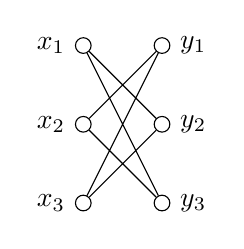
\begin{tikzpicture}
\node [draw, fill=white, circle, inner sep=2pt, label=left:{$x_3$}] (x3) at (0,0) {};
\node [draw, fill=white, circle, inner sep=2pt, label=left:{$x_2$}] (x2) at (0,1) {};
\node [draw, fill=white, circle, inner sep=2pt, label=left:{$x_1$}] (x1) at (0,2) {};
\node [draw, fill=white, circle, inner sep=2pt, label=right:{$y_3$}] (y3) at (1,0) {};
\node [draw, fill=white, circle, inner sep=2pt, label=right:{$y_2$}] (y2) at (1,1) {};
\node [draw, fill=white, circle, inner sep=2pt, label=right:{$y_1$}] (y1) at (1,2) {};

\draw (x1)--(y2)--(x3)--(y1)--(x2)--(y3)--(x1);
\end{tikzpicture}
&\ \hspace{2cm}\ &
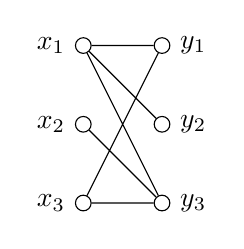
\begin{tikzpicture}
\node [draw, fill=white, circle, inner sep=2pt, label=left:{$x_3$}] (x3) at (0,0) {};
\node [draw, fill=white, circle, inner sep=2pt, label=left:{$x_2$}] (x2) at (0,1) {};
\node [draw, fill=white, circle, inner sep=2pt, label=left:{$x_1$}] (x1) at (0,2) {};
\node [draw, fill=white, circle, inner sep=2pt, label=right:{$y_3$}] (y3) at (1,0) {};
\node [draw, fill=white, circle, inner sep=2pt, label=right:{$y_2$}] (y2) at (1,1) {};
\node [draw, fill=white, circle, inner sep=2pt, label=right:{$y_1$}] (y1) at (1,2) {};

\draw (y2)--(x1)--(y1)--(x3)--(y3)--(x1) (x2)--(y3);
\end{tikzpicture}\\
\end{tabular}
\caption{دو مثال از گراف‌های دوبخشی}
\label{figure: bipartite graph}
\end{figure}


\begin{latin}
\begin{algorithm}[H]
\begin{algorithmic}[1]\baselineskip=10pt\relax

\REQUIRE A labeled bipartite graph $ \Gamma $ with bipartition $ X, Y $
\ENSURE A positive matching decomposition of $ \Gamma $
\STATE $ k\longleftarrow 0 $
\WHILE{$ E(\Gamma) \neq \varnothing $}
\STATE $ k \longleftarrow k + 1 $
\STATE  $ X' \longleftarrow X \setminus \{\text{isolated vertices of } X\}$
\STATE  $ Y' \longleftarrow \varnothing $
\STATE $M_k \longleftarrow \varnothing $
\WHILE{$ X' \neq \varnothing$}
\STATE $ s \longleftarrow \min(\text{Slopes}(\Gamma[X'\cup Y])) $
\STATE $ M \longleftarrow \{xy \in E(\Gamma[X'\cup Y]) \colon \quad \mathrm{slope}(xy)=s\} $
\STATE $ M_k \longleftarrow M_k \cup \{xy \in M \colon \quad y \notin Y'\} $
\STATE $ X' \longleftarrow X' \setminus \{x \colon \quad xy\in M\} $
\STATE $ Y' \longleftarrow Y' \cup \{y \colon \quad xy\in M\} $
\ENDWHILE
\STATE $E(\Gamma) \longleftarrow E(\Gamma) \setminus M_k $
\ENDWHILE
\RETURN $ M_1,\ldots,M_k$

\end{algorithmic}
\caption{\textsc{A positive matching decomposition of a labeled bipartite graph}}
\label{alg:A positive matching decomposition of a labeled bipartite graph}
\end{algorithm}
\end{latin}

\begin{latin}
\begin{table}[H]
\begin{tabular}{|c|c|c|>{\centering}p{3cm}|>{\centering}p{4cm}|}
\cline{3-5}
\multicolumn{2}{c}{} & \multicolumn{2}{|c|}{Oriented surfaces} & {Non-oriented surfaces} \tabularnewline
\cline{2-5}
\multicolumn{1}{c|}{} & {\multirow{2}{*}{$S$}} & {\multirow{2}{*}{Sphere}} & Connected sum of {$r$ tori} & Connected sum of $r$ Projective Plane \tabularnewline
%\multicolumn{1}{c|}{} &  &  & {$r$ tori} & $r$ Projective Plane \\
\cline{2-5}
\multicolumn{1}{c|}{} & $\chi(S)$ & $2$ & $2-2r$ & $ 2-r $ \tabularnewline
\hline
{\multirow{3}{*}{$\tilde{H}_i(S,\mathbb{K})$}} & $i=0$ & $0$ & $0$ & $0$ \tabularnewline
\cline{2-5}
 & $i=1$ & $0$ & $\mathbb{K}^{2r}$ & $(\mathbb{Z}_2 \otimes_\mathbb{Z} \mathbb{K}) \oplus \mathbb{K}^{r-1}$ \bigstrut\tabularnewline
\cline{2-5}
 & $i=2$ & $\mathbb{K}$ & $\mathbb{K}$ & $\mathrm{Tor}_{1}^{\mathbb{Z}}(\mathbb{Z}_2,\mathbb{K})$ \bigstrut\tabularnewline
\hline
\end{tabular}
\caption{Homology of $2$-manifolds}
\label{Table of Homology}
\end{table}
\end{latin} % if any un-wanted empty page is produced between chapters, you can use \input instead of \include : \chapter{عنوان فصل یا پیوست}

به‌عنوان مثال مقداری متن در این قسمت قرار می‌دهیم. فرض کنید $\mathbb{K}$ یک میدان و $S=\mathbb{K}[x_1, \ldots, x_n]$ حلقه چندجمله‌ای‌ها روی میدان $\mathbb{K}$ باشد که با درجه‌بندی استاندارد مدرج شده است. فرض کنید $M = \oplus_{i\in \mathbb{Z}}M_i$ یک $S$-مدول ناصفر با تولید متناهی باشد. به ازای هر $i \in \mathbb{N} \cup \{0\}$، تعریف می‌کنیم:
\[t^S_i(M) = \max \{j \colon \quad \beta^\mathbb{K}_{i,j}(M) \neq 0\} \]
که در آن $\beta^\mathbb{K}_{i,j}(M)$، همان $i,j$-امین عدد بتی $M$ به عنوان $S$-مدول است. در واقع
\[\beta^\mathbb{K}_{i,j}(M) = \dim_\mathbb{\mathbb{K}} \mathrm{Tor}_{i}^{S}(\mathbb{\mathbb{K}},M)_j\]
در حالتی که $\mathrm{Tor}_{i}^{S}(\mathbb{\mathbb{K}},M)=0$، قرار می‌دهیم $t^S_i(M)= - \infty$.

عدد نظم کاستلنوو-مامفورد $M$ که با $\mathrm{reg}(M)$ نمایش  می‌دهیم را به صورت زیر تعریف  می‌کنیم:
\[\mathrm{reg} (M)= \sup \{t^S_i(M)-i \colon \quad i \in \mathbb{Z} \}.\]

همچنین درجه آغازین یک $S$-مدول با تولید متناهی و ناصفر $M= \oplus_{i\in \mathbb{Z}}M_i$ را با $\mathrm{indeg}\, (M)$ نمایش داده و به صورت زیر تعریف  می‌کنیم:
\[\mathrm{indeg}\, (M)=\inf \{i \colon \quad M_i \neq 0 \}.\]
گوییم $M$ دارای تحلیل $d$-خطی است، هرگاه 
$\mathrm{reg}(M)=\mathrm{indeg}\,(M)$.

\begin{theorem} 
فرض کنید $M \neq 0$ یک $S$-مدول با تولید متناهی باشد. موارد زیر هم‌ارز هستند:
\begin{itemize}
\item[(آ)] $a = \mathrm{reg} (M)$.
\item[(ب)] $a = \max\{t \colon \quad \beta^\mathbb{\mathbb{K}}_{i,i+t}(M) \neq 0; \quad i \geq 0 \text{به‌ازای برخی } \}$.
\item[(پ)] $a = \max \{t \colon \quad \mathrm{Tor}_{i}^{S}(K,M)_{t+i} \neq 0; \quad i \geq 0 \text{به‌ازای برخی } \}$.
\item[(ت)] $a = \max \{t \colon \quad \mathrm{Ext}_{S}^{i}(K,M)_{-t-i} \neq 0; \quad i \geq 0 \text{به‌ازای برخی } \}$.
\item[(ث)] $a = \max \{t \colon \quad  {H_\mathfrak{m}^i(M)}_{t-i} \neq 0; \quad i \geq 0 \text{به‌ازای برخی } \}$.
\item[(ج)] $a = \max \{a_i(M)+i \colon \quad i \in \mathbb{N} \}$ که در آن  $a_i(M)= \max \{t \colon \quad {H_\mathfrak{m}^i (M)}_{t} \neq 0 \}$.
\end{itemize}
\end{theorem}

\section{عنوان بخش }
متن بخش اول را در اینجا بنویسید.
\begin{definition}
فرض کنید $[n]=\{1, \ldots,n\}$ و $\Delta$ یک مجتمع سادکی بر $[n]$ باشد. دراین‌صورت ایدآل استنلی-رایزنر $\Delta$ را با $I_\Delta$ نمایش داده و به‌صورت زیر تعریف می کنیم
\[I_\Delta=(\mathbf{x}_F \colon \quad F \notin \Delta).\]
\end{definition}

\subsection{عنوان زیر بخش }

\begin{theorem}\label{Resolution of minimal}
فرض کنید $\mathcal{C}$ یک $d$-ابرگراف روی مجموعه رأس‌های $[n]$ باشد که مینیمال نسبت به $d$-خطی‌بودن است و 
 $I=I(\bar{\mathcal{C}}) \subset \mathbb{K}[x_1, \ldots, x_n]$ 
  ایدآل متناظر با 
 $\mathcal{C}$
  باشد. در این‌صورت تحلیل آزاد مینیمال ایده‌آل
  $I$
   به صورت زیر است:
\begin{align*} 
0  \to S^{\beta_{n-d,n}}(-n) & \to S(-n) \oplus S^{\beta_{n-d-1, n-1}}(-(n-1)) \to  S^{\beta_{n-d-2, n-2}}(-(n-2))  \\
& \to \cdots \to S^{\beta_{1,d+1}}(-(d+1)) \to S^{\beta_{0,d}}(-d) \to I \to 0 \label{Resolution of Minimal to linearity+Shape}
\end{align*}
که در آن،
\begin{itemize}
\item[(آ)] 
$\beta_{n-d,n}(I) = 1 -e(S/I) + \sum\limits_{i=0}^{d-1} (-1)^{d+i-1} {n \choose i}$.
\item[(ب)]
برای $0 \leq i \leq n-d-1$، داریم 
$\beta_{i, i+d}(I) = {n-d \choose i} \left( \frac{d}{d+i}{n \choose d} - e(S/I) \right)$.
\end{itemize}

\end{theorem}

\begin{example}[رجوع شود به {\cite[{قضیه 5.3}]{Morales_Pour_Zaare-Nahandi_2016}}]
فرض کنید $\Delta$ یک مثلث‌بندی از کره $\mathbb{S}^2$ با $n>4$ رأس باشد و $\mathcal{C}=\mathcal{F}(\Delta)$، ابرگراف متناظر با $\Delta$ باشد. دراین‌صورت $\mathcal{C}$ یک $3$-شبه‌منیفلد جهت‌پذیر است. پس با توجه به قضیه، ابرگراف $\mathcal{C}$ مینیمال نسبت به $3$-خطی‌بودن است. لذا قضیه \ref{Resolution of minimal} ایجاب می‌کند که تحلیل آزاد مینیمال ایدآل   $I=I(\bar{\mathcal{C}})$  به صورت زیر است:
\begin{align*} 
0 \to S^{\beta_{n-3,n}}(-n) \to S(-n) \oplus S^{\beta_{n-4, n-1}}(-(n-1)) \to  S^{\beta_{n-5, n-2}}(-(n-2)) \\
 \to \cdots \to S^{\beta_{0,3}}(-3) \to I \to 0
\end{align*}
که در آن،
\[\beta^\mathbb{K}_{i, i+3}(I) = {n-3 \choose i} \left( \frac{3}{3+i}{n \choose 3} - 2(n-2) \right).\]

\end{example}
\section{بخش دوم}
\begin{proposition}
مقداری متن مقداری متن مقداری متن مقداری متن مقداری متن 
\end{proposition}



\begin{corollary}
مقداری متن مقداری متن مقداری متن مقداری متن مقداری متن 
\end{corollary}



\begin{lemma}
مقداری متن مقداری متن مقداری متن مقداری متن مقداری متن 
\end{lemma}



\begin{conjecture}
مقداری متن مقداری متن مقداری متن مقداری متن مقداری متن 
\end{conjecture}


\begin{remark}
مقداری متن مقداری متن مقداری متن مقداری متن مقداری متن 
\end{remark}


\begin{question}
مقداری متن مقداری متن مقداری متن مقداری متن مقداری متن 
\end{question}


\begin{problem}
مقداری متن مقداری متن مقداری متن مقداری متن مقداری متن 
\end{problem}


\begin{notation}
مقداری متن مقداری متن مقداری متن مقداری متن مقداری متن 
\end{notation}




\begin{figure}[h]
\centering
\begin{tabular}{ccc}
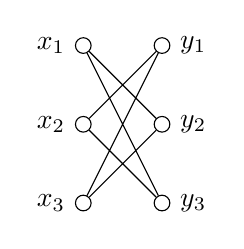
\begin{tikzpicture}
\node [draw, fill=white, circle, inner sep=2pt, label=left:{$x_3$}] (x3) at (0,0) {};
\node [draw, fill=white, circle, inner sep=2pt, label=left:{$x_2$}] (x2) at (0,1) {};
\node [draw, fill=white, circle, inner sep=2pt, label=left:{$x_1$}] (x1) at (0,2) {};
\node [draw, fill=white, circle, inner sep=2pt, label=right:{$y_3$}] (y3) at (1,0) {};
\node [draw, fill=white, circle, inner sep=2pt, label=right:{$y_2$}] (y2) at (1,1) {};
\node [draw, fill=white, circle, inner sep=2pt, label=right:{$y_1$}] (y1) at (1,2) {};

\draw (x1)--(y2)--(x3)--(y1)--(x2)--(y3)--(x1);
\end{tikzpicture}
&\ \hspace{2cm}\ &
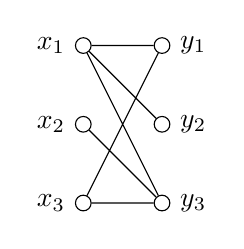
\begin{tikzpicture}
\node [draw, fill=white, circle, inner sep=2pt, label=left:{$x_3$}] (x3) at (0,0) {};
\node [draw, fill=white, circle, inner sep=2pt, label=left:{$x_2$}] (x2) at (0,1) {};
\node [draw, fill=white, circle, inner sep=2pt, label=left:{$x_1$}] (x1) at (0,2) {};
\node [draw, fill=white, circle, inner sep=2pt, label=right:{$y_3$}] (y3) at (1,0) {};
\node [draw, fill=white, circle, inner sep=2pt, label=right:{$y_2$}] (y2) at (1,1) {};
\node [draw, fill=white, circle, inner sep=2pt, label=right:{$y_1$}] (y1) at (1,2) {};

\draw (y2)--(x1)--(y1)--(x3)--(y3)--(x1) (x2)--(y3);
\end{tikzpicture}\\
\end{tabular}
\caption{دو مثال از گراف‌های دوبخشی}
\label{figure: bipartite graph}
\end{figure}


\begin{latin}
\begin{algorithm}[H]
\begin{algorithmic}[1]\baselineskip=10pt\relax

\REQUIRE A labeled bipartite graph $ \Gamma $ with bipartition $ X, Y $
\ENSURE A positive matching decomposition of $ \Gamma $
\STATE $ k\longleftarrow 0 $
\WHILE{$ E(\Gamma) \neq \varnothing $}
\STATE $ k \longleftarrow k + 1 $
\STATE  $ X' \longleftarrow X \setminus \{\text{isolated vertices of } X\}$
\STATE  $ Y' \longleftarrow \varnothing $
\STATE $M_k \longleftarrow \varnothing $
\WHILE{$ X' \neq \varnothing$}
\STATE $ s \longleftarrow \min(\text{Slopes}(\Gamma[X'\cup Y])) $
\STATE $ M \longleftarrow \{xy \in E(\Gamma[X'\cup Y]) \colon \quad \mathrm{slope}(xy)=s\} $
\STATE $ M_k \longleftarrow M_k \cup \{xy \in M \colon \quad y \notin Y'\} $
\STATE $ X' \longleftarrow X' \setminus \{x \colon \quad xy\in M\} $
\STATE $ Y' \longleftarrow Y' \cup \{y \colon \quad xy\in M\} $
\ENDWHILE
\STATE $E(\Gamma) \longleftarrow E(\Gamma) \setminus M_k $
\ENDWHILE
\RETURN $ M_1,\ldots,M_k$

\end{algorithmic}
\caption{\textsc{A positive matching decomposition of a labeled bipartite graph}}
\label{alg:A positive matching decomposition of a labeled bipartite graph}
\end{algorithm}
\end{latin}

\begin{latin}
\begin{table}[H]
\begin{tabular}{|c|c|c|>{\centering}p{3cm}|>{\centering}p{4cm}|}
\cline{3-5}
\multicolumn{2}{c}{} & \multicolumn{2}{|c|}{Oriented surfaces} & {Non-oriented surfaces} \tabularnewline
\cline{2-5}
\multicolumn{1}{c|}{} & {\multirow{2}{*}{$S$}} & {\multirow{2}{*}{Sphere}} & Connected sum of {$r$ tori} & Connected sum of $r$ Projective Plane \tabularnewline
%\multicolumn{1}{c|}{} &  &  & {$r$ tori} & $r$ Projective Plane \\
\cline{2-5}
\multicolumn{1}{c|}{} & $\chi(S)$ & $2$ & $2-2r$ & $ 2-r $ \tabularnewline
\hline
{\multirow{3}{*}{$\tilde{H}_i(S,\mathbb{K})$}} & $i=0$ & $0$ & $0$ & $0$ \tabularnewline
\cline{2-5}
 & $i=1$ & $0$ & $\mathbb{K}^{2r}$ & $(\mathbb{Z}_2 \otimes_\mathbb{Z} \mathbb{K}) \oplus \mathbb{K}^{r-1}$ \bigstrut\tabularnewline
\cline{2-5}
 & $i=2$ & $\mathbb{K}$ & $\mathbb{K}$ & $\mathrm{Tor}_{1}^{\mathbb{Z}}(\mathbb{Z}_2,\mathbb{K})$ \bigstrut\tabularnewline
\hline
\end{tabular}
\caption{Homology of $2$-manifolds}
\label{Table of Homology}
\end{table}
\end{latin}

\chapter{مفاهیم بنیادی}

\section{مقدمه}
در این فصل، مفاهیم بنیادی و پیش‌نیازهایی که برای درک بهتر پژوهش حاضر ضروری هستند معرفی می‌شوند. از آنجا که این پایان‌نامه در تقاطع علوم زیستی و روش‌های محاسباتی قرار دارد، آشنایی با مفاهیم هر دو حوزه برای دنبال‌کردن مطالب فصل‌های بعدی اهمیت ویژه‌ای دارد.
بر همین اساس، در بخش نخست این فصل، مفاهیم زیستی مرتبط با موضوع پژوهش مورد بررسی قرار می‌گیرند. سپس در بخش دوم، به معرفی مفاهیم محاسباتی مورد استفاده پرداخته می‌شود و تمرکز اصلی بر مباحث مرتبط با شبکه‌های عصبی گرافی و چارچوب‌های یادگیری مبتنی بر گراف خواهد بود.
در نهایت، در بخش پایانی این فصل، معیارهای ارزیابی به‌کاررفته در این پژوهش برای سنجش کیفیت شناسایی ماژول‌های عملکردی معرفی شده و به‌طور خلاصه تشریح می‌شوند تا زمینه لازم برای تحلیل نتایج در فصل‌های بعدی فراهم شود.

\section{مفاهیم زیستی}
مقدمه کوچک
\subsection{پروتئین}
\subsection{ماژول‌های عملکردی}
\subsection{شبکه‌های PPI}
\subsection{هستی شناسی ژن}
\subsection{بیان ژن}


\section{مفاهیم محاسباتی}

در مفاهیم بنیادی ابتدا به فرمول بندی مسئله خوشه‌بندی گراف‌های با گره‌های دارای ویژگی می‌پردازیم. 

\subsection{خوشه بندی در گراف های با گره های دارای ویژگی }
با فرض گراف $G=(V,E,F)$ که در آن $V$ مجموعه گره ها، $E$ مجموعه یال ها است و $F$ ماتریس ویژگی های گره ها می باشد، یک خوشه بندی از گراف $G$ را می توان با $C$ نشان داد که مجموعه ای از زیر مجموعه های $V$ است، به صورتی که  $C_i\in C\:;\:C_i\subset V$. هدف از خوشه بندی این است که خوشه هایی که هم از نظر ساختاری و هم از نظر ویژگی های گره‌ها بهم بیشترین شباهت را دارند، پیدا کنیم. همچنین خوشه‌های ایجاد شده باید از نظر ارتباط‌ یال‌های داخل خوشه چگال و در ارتباط یال‌ها با دیگر خوشه‌ها تنک باشند.

\subsection{دسته‌بندی و روش‌های کلی خوشه‌بندی گراف}
 روش‌های خوشه‌بندی گراف را می‌توان از دیدگاه‌های مختلفی تقسیم‌بندی کرد. این تقسیم‌بندی‌ها بر اساس معیارها و ویژگی‌های خاصی صورت می‌گیرند که به نحوه برخورد با داده‌های گرافی، نوع اطلاعات استفاده شده، و تکنیک‌های به کار گرفته شده بستگی دارد. در این پژوهش از آنجایی که نوع گراف ورودی مشخص است و قصد خوشه‌بندی گراف‌های \lr{PPI} با گره‌های دارای ویژگی را داریم، روش‌های خوشه‌ بندی را بر اساس روش‌ مورد استفاده تقسیم‌بندی می‌کنیم:

\begin{itemize}
    \item روش‌های طیفی\footnote{\lr{Spectral clustering}} : از مقادیر ویژه\footnote{\lr{Eigenvalues }}  ماتریس لاپلاسین یا مجاورت برای یافتن خوشه‌ها استفاده می‌کنند.
    \item روش‌های فاکتورگیری ماتریسی\footnote{\lr{Matrix factorization}} : از روش‌های تجزیه‌ ماتریسی مانند تجزیه نامنفی ماتریس\footnote{\lr{Non-negative matrix factorization}}  یا تجزیه مقدار تکین\footnote{\lr{Singular value factorization}}  برای ایجاد امبدینگ و خوشه‌بندی استفاده می‌کنند.
    \item روش‌های سلسله‌مراتبی\footnote{\lr{Hierarchical clustering}} : گراف را به صورت سلسله ‌مراتبی خوشه‌بندی می‌کنند که به دو روش تقسیمی و تجمعی دسته‌بندی می‌شوند.
    \item روش‌های مبتنی بر امبدینگ\footnote{\lr{Embedding-based methods}} : ابتدا گره‌ها به فضای برداری کم‌بعد نگاشت می‌شوند و سپس خوشه‌بندی روی این فضای برداری انجام می‌شود و تمرکز اصلی در این روش‌ها یافتن بازنمایی مناسب برای خوشه‌بندی گراف است. \lr{(Node2Vec, DeepWalk, GCN, GNN)}.
    \item روش‌های بدون امبدینگ\footnote{\lr{Non-embedding methods}} : مستقیماً از ساختار گراف برای خوشه‌بندی استفاده می‌شود بدون اینکه گره‌ها به فضای برداری منتقل شوند \lr{(Louvain, graph - cut based)}.

\end{itemize}

\subsection{پایگاه داده هستی شناسی ژن}
\lr{GO} یک بانک داده و سیستم طبقه‌بندی است که با هدف ایجاد یک زبان استاندارد برای توصیف ژن‌ها و محصولات ژنی (که پروتئین‌ها نیز جزو آنها هستند) ایجاد شده است. این سیستم شامل سه بخش اصلی است که هر یک از آنها یک جنبه خاصی از عملکرد زیستی را توصیف می‌کنند:

فرآیند زیستی\footnote{\lr{Biological process}} : این بخش به فرآیند‌های زیستی اشاره دارد که ژن و یا پروتئین خاصی در آن نقش دارد.

عملکرد مولکولی\footnote{\lr{Molecular function}} : این بخش عملکرد دقیق مولکولی ژن یا پروتئین را توصیف می‌کند.

مولفه‌ی سلولی\footnote{\lr{Cellular component}} : این بخش به مکانی که ژن یا پروتئین در آن قرار دارد اشاره می‌کند.
از ویژگی‌های دیگر این بانک داده نمایش اطلاعات به صورت سازماندهی شده و سلسله مراتبی است که شامل شبکه‌های بدون دور می‌شود و ویژگی‌ها به این صورت مرتب شده‌اند \cite{gene}. 

\subsection{شبکه‌های PPI و ویژگی‌های آنها }
یک شبکه \lr{PPI} معمولا به صورت یک گراف بدون جهت $G=(V,E)$ نشان داده می شود که $V$ و $E$ به ترتیب نمایان‌گر پروتئین ها و تعاملات بین آنها می باشند. وزن های روی یال ها را می توان برای توصیف ویژگی های شبکه \lr{PPI}، مانند ویژگی‌های توپولوژیکی یا عملکردی استفاده کرد. شبکه های \lr{PPI} سه ویژگی توپولوژیکی زیر را دارند:

\begin{itemize}
    \item توزیع بدون مقیاس\footnote{\lr{Scale-free distribution}} : $P(k)$   مفهوم توزیع درجه یعنی احتمال اینکه یک گره در یک شبکه دقیقا \lr{k} پیوند داشته باشد را نشان می دهد. یک  شبکه \lr{PPI} دارای توزیع درجه توانی $P(k)\sim\:k^{-\lambda}$ می باشد\cite{evolution} . این ویژگی به این معنی است که پروتئین‌های تعامل‌دار در شبکه‌های \lr{PPI} به طور یکنواخت توزیع نمی شوند‌، بیشتر پروتئین‌ها تنها در چند تعامل شرکت می‌کنند در حالی که مجموعه کوچکی از پروتئین‌ها در ده‌ها تعامل (تشکیل گره هاب\footnote{\lr{Hub}}) شرکت می‌کنند. 
    \item ویژگی جهان کوچک\footnote{\lr{Small-world property}} : پروتئین‌های یک شبکه \lr{PPI} دارای میانگین طول مسیر کم و ضرایب خوشه‌ای بالا هستند\cite{protein}  که سیگنال‌های هر گره در شبکه \lr{PPI} را قادر می‌سازد تا از طریق چند جهش به سرعت به هر گره دیگری برسند. در نتیجه شبکه‌های \lr{PPI} هم زمان انتقال سیگنال و هم زمان پاسخ کوتاهی خواهند داشت.
    \item شبکه با ماژول‌های عملکردی\footnote{\lr{Functional modular network}} : شبکه \lr{PPI} یک شبکه ماژولار و سلسله مراتبی می‌باشد. یک ماژول عملکردی در یک شبکه \lr{PPI} یک مجموعه با بیشترین تعداد پروتئین که عملکرد یکسانی دارند، می‌باشد. بارزترین مشخصه ماژول عملکردی، ارتباط بین ساختار توپولوژیکی شبکه \lr{PPI} و عملکرد‌ پروتئین‌های آن است که مبنای بسیاری از روش‌های تشخیص ماژول عملکردی است\cite{molecular} \cite{road}.
\end{itemize}


\chapter{بررسی منابع}
در این قسمت به بررسی پژوهش‌های پیشینی که به منظور پیدا کردن مجموعه‌های پروتئینی در شبکه‌های \lr{PPI} انجام شده‌اند، می‌پردازیم. همانطور که در بخش‌های پیشین بررسی شد، تمرکز این پژوهش بر روی دید گرافی به شبکه‌های \lr{PPI} و ادغام اطلاعات زیست‌شناسی پروتئین‌ها به منظور تشخیص دقیق‌تر مجموعه‌های پروتئینی است. از آنجایی که پیدا کردن مجموعه‌های پروتئینی در شبکه‌های \lr{PPI} معادل خوشه‌بندی این شبکه‌ها می‌باشد، ما ابتدا چند نمونه از پژوهش‌های مرتبط با خوشه‌بندی گراف‌های دارای گره‌ ویژگی که بیشترین ارتباط را با هدف پژوهش ما دارند را بررسی می‌کنیم. 
\section{خوشه‌بندی گراف‌های دارای گره ویژگی}
پژوهش وحید جان‌نثاری و همکارانش\cite{nonnegative} ، یک الگوریتم بر پایه تجزیه نامنفی ماتریسی\footnote{\lr{Non-negative matrix factorization}}  به منظور خوشه‌بندی گراف‌های ویژگی‌دار معرفی می‌کند. روش آن‌ها ابتدا اطلاعات ساختاری که توسط ماتریس همسایگی\footnote{\lr{Adjacency matrix}}  نشان داده می‌شود را به کمک تجزیه نامنفی متقارن ماتریس\footnote{\lr{Symmetric non-negative matrix factorization}}  و اطلاعات ویژگی‌های گره‌ها را به کمک تجزیه نامنفی بازتابی ماتریس\footnote{\lr{Projective non-negative matrix factorization}}  به یک فضای کم بعد مختص خوشه‌بندی (هم بعد با تعداد خوشه‌ها) به صورت جداگانه انتقال می‌دهد که درجه عضویت هر گره به هر خوشه را نمایش می‌دهد. همینطور به منظور حفظ ثبات در خوشه بندی در هر دو فضا اقدام به نزدیک کردن این دو ماتریس به کمک تابع هدف می‌کند که به صورت مقابل تعریف شده است:
\begin{gather}
    J_{of}=min||A-VV^{T}||_{F}^{2}+\alpha||VV^{T}-UU^{T}||_{F}^{2}+||F-UU^{T}F||_{F}^2 \\
    s.t.\:\: V\ge 0,\: U\ge 0,\:V^TV=I,\: U^TU=I.\nonumber  
\end{gather}

که در تابع هدف، \lr{A} ماتریس همسایگی، $V\in R^{n\times k}$ ماتریس حاصل از تجزیه نامنفی متقارن ماتریس \lr{A} است. همینطور با در نظر  گرفتن \lr{M} (ماتریس شباهت\footnote{\lr{Similarity matrix}}  گره‌ها براساس ماتریس ویژگی‌ها) به صورت $M=UU^T;U\in R^{n\times k}$ و عبارت سوم در بهینه سازی که به صورت مقابل بیان شده است:  $|F-MF|$ در واقع اقدام به استفاده از ویژگی خودبیانگری\footnote{\lr{Self-expression }}  داده‌ها کرده‌اند، که در نتیجه روش بیان شده را می‌توان یک روش ترکیبی از خوشه‌بندی زیر فضا\footnote{\lr{Subspace clustering}}  و تجزیه نامنفی ماتریس در نظر گرفت.

در پژوهشی دیگر توسط کانگ و همکارانش\cite{fine} ، یک روش بر پایه شبکه‌های پیچشی گرافی\footnote{\lr{Graph convolutional networks}}  و خوشه‌بندی طیفی ارائه شده است. ایده اصلی در این روش بر پایه پردازش سیگنالی گراف است که در آن یک فیلتر پایین گذر\footnote{\lr{Low-pass filter}}  را به منظور نزدیک کردن و ادغام ویژگی‌های گره‌ها و ساختار گراف به ماتریس ویژگی‌ها اعمال می‌کنند. در نتیجه یک بازنمایی جدید بر این اساس را برای گره‌ها بدست می‌آورند:
\begin{equation}
\bar{X}=(I-1/2 L)^k X    
\end{equation}

همچنین در فرمول بالا \lr{k} یک هایپر پارامتر است که میزان مرتبه مجاورت بازنمایی به دست آمده را مشخص می‌کند به عبارت دیگر مقادیر کوچک‌تر \lr{k} دید محلی تری به ساختار گراف دارند و بالعکس. $L=I-A$ که \lr{L}  ماتریس لاپلاسی نرمال شده\footnote{\lr{Normalized Laplacian matrix}}  می‌باشد. در مرحله بعد برای اعمال خوشه‌بندی طیفی، نیاز به محاسبه ماتریس شباهت بین گره‌ها است که به صورت مقابل عمل کرده‌اند.

\begin{equation}
\min_S||\bar{X} ^T- \bar{X} ^T S||_F^2+α||S-f(A)||_F^2    
\end{equation}


که در اینجا ماتریس شباهت \lr{S} از بهینه سازی تابع هدف بالا بدست می‌آید و سپس با یک انتقال به یک ماتریس متقارن نامنفی تبدیل شده و در نهایت نیز خوشه‌بندی طیفی روی آن اعمال می‌شود. یکی از مشکلات این روش انتخاب مناسب هایپر پارامتر \lr{K} است که به طور مستقیم بر خروجی الگوریتم تاثیر می‌گذارد که توسط پژوهش دیگری که توسط ژانگ و همکارانش\cite{adaptive}  انجام شده‌ است، دو استراتژی \lr{AGC} و \lr{IAGC} برای پیدا کردن مقدار مناسب \lr{k} ارائه شده است.

یکی از مشکلات روش‌های بر پایه بازنمایی این است که دو فرآیند بازنمایی‌ها داده‌ها و خوشه‌بندی از یکدیگر مستقل‌اند در نتیجه نمی‌توان اطمینان داشت که بازنمایی‌های ایجاد شده برای وظیفه مورد‌نظر (در اینجا خوشه‌بندی) مناسب هستند و همچنین نمی‌توان الگوریتم بازنمایی را بر اساس خطای خوشه‌بندی به طور مناسب به روزرسانی نمود. از این روی، وانگ و همکاران\cite{2019attributed}  یک روش خوشه بندی یکپارچه توجه محور بر پایه شبکه عصبی گراف ارائه داده‌اند که مرحله بازنمایی و خوشه‌بندی را با هم ترکیب می‌کند. در این پژوهش از یک شبکه گرافی توجه محور\footnote{\lr{Graph attentional}}  به عنوان کدگذار  استفاده شده‌ است. ضرایب توجه کدگذار\footnote{\lr{Decoder}} با استفاده از یک ماتریس مجاورت با مرتبه بالا همانند پژوهش قبلی محاسبه می‌شوند. قسمت کدگشا\footnote{\lr{Encoder}}  نیز از ضرب داخلی بردار‌های بازنمایی کدگذار به منظور بازسازی ماتریس مجاورت گراف استفاده می‌کند که برای خروجی این قسمت تابع هزینه بازسازی در نظر گرفته شده است. نوآوری این مقاله در معرفی مفهوم بازنمایی خود بهینه‌ساز است که در آن به طور مکرر نقاط مربوط به هر خوشه براساس مقدار اطمینان تعلق به خوشه به‌روزرسانی می‌شود و به طور همزمان بازنمایی‌ها را نیز به وسیله آن اصلاح می‌کند.

\section{پیش‌بینی مجموعه‌های پروتئینی}

در ادامه به بررسی روش‌های استفاده شده به منظور پیش‌بینی مجموعه‌های پروتئینی در شبکه‌های \lr{PPI} می‌پردازیم و یک دسته‌بندی برای این روش‌ها ارائه می‌دهیم. به طور کلی الگوریتم‌های پیش‌بینی مجموعه‌های پروتئینی را می‌توان به دو دسته تقسیم کرد:

\textbf{روش‌های بر پایه شبکه \footnote{\lr{Network-based methods}}: }\\
این روش‌ها تنها بر ساختار شبکه \lr{PPI} تمرکز می‌کنند. که به دو زیر دسته تقسیم می‌شوند:
\begin{itemize}
    \item روش‌های تقسیمی \footnote{\lr{Divisive methods }}: این دسته از روش‌ها، شبکه را به زیر شبکه‌ها تقسیم می‌کنند و این عمل را تا رسیدن به درجه دلخواه خوشه بندی تکرار می‌کنند. معروف ترین الگوریتم‌ این دسته الگوریتم خوشه‌بندی مارکوف\footnote{\lr{Markov clustering algorithm}}  \cite{2012markov} است که زیر شبکه‌ها را به کمک قدم تصادفی\footnote{\lr{Random walk}}  در شبکه پیدا می‌کند.
    \item روش‌های تجمعی \footnote{\lr{Agglomerative methods}}: با مجموعه کوچکی از پروتئین‌ها شروع کرده و با ترکیب آن‌ها اقدام به پیدا کردن مجموعه‌های پروتئینی نهایی می‌کند. الگوریتم \lr{CPNM} \cite{2020motif} یکی از الگوریتم‌‌های این دسته است که از امبدینگ موتیف‌های\footnote{\lr{Motif}}  شبکه به منظور پیدا کردن نقش پروتئین‌ها استفاده می‌کند. سپس به منظور ایجاد بردار ویژگی‌ پروتئین‌ها از آن‌ها استفاده می‌شود. در نهایت نیز از روش پیدا کردن همسایگان به منظور شناسایی مجموعه‌های پروتئینی استفاده می‌کند. یکی دیگر از الگوریتم‌های تجمعی معروف الگوریتم \lr{ClusterONE} \cite{2012clusterone} است. این الگوریتم ابتدا پروتئین‌های با درجه‌ بالاتر را به عنوان پروتین‌های هسته \footnote{\lr{Seed}} (پروتین‌های آغازین)‌ در نظر گرفته می‌گیرد. سپس زیرگروه‌هایی از گره‌ها با بیشترین انسجام برای گره‌های هسته انتخاب می‌شوند. در انتها نیز گره هسته از بین گره‌هایی که مربوط به یک ترکیب شناخته شده نیستند انتخاب می‌شوند و این مراحل تکرار می‌شوند تا همه پروتئین‌ها به یک ترکیب مرتبط شوند. الگوریتم دیگر، \lr{MCODE}\footnote{\lr Molecular complex detection}  \cite{2003mcode} است که در سه مرحله انجام می‌شود. این الگوریتم ابتدا گره‌ها را وزن دهی می‌کند، سپس به شناسایی مجموعه‌ها می‌پردازد و در انتها نیز اقدام به اضافه / حذف کردن پروتئين‌ها به/از مجموعه‌های شناسایی شده با توجه به یک معیار اتصال می‌کند.
\end{itemize}

\textbf{روش‌های مبتنی بر آگاهی از زمینه‌های زیستی \footnote{\lr{Biological-context-aware-based methods}}:}\\
اگرچه روش‌های بر پایه شبکه عملکرد خوبی دارند، اما عملکرد آنها می‌تواند با به کارگیری اطلاعات تکمیلی بهبود یابد. این اطلاعات می‌توانند از منابع گوناگونی مثل اطلاعات دامنه‌ای پروتئین‌ها، برچسب‌های ژن شناسی، نمایه بیان ژنی جمع آوری شوند. پژوهش آلن و همکارانش \cite{2013PCIA}، الگوریتم \lr{PCIA} را توسعه داده‌اند که از ترکیب اطلاعات \lr{GO} در کنار ساختار شبکه استفاده می‌کند.  پژوهش دیگر ژانگ و همکارانش \cite{2019integrating} رابطه‌ی بین شکل گیری مجموعه‌های پروتئینی و هم بیانی پروتئین‌ها را نشان داده است.
\begin{itemize}
    \item روش‌های هسته-اتصال \footnote{\lr{Core-attachment}}: روش‌های هسته-اتصال بر پایه این ایده هستند که هر مجموعه پروتئینی از یک هسته تشکیل شده‌ است که شامل پروتئین‌هایی با هم بیانی بالا می‌باشند. الگوریتم \lr{COACH} \cite{2009core} یکی از شناخته شده‌ترین الگوریتم‌های این دسته است که از دو مرحله شناسایی پروتئین‌های هسته‌ای و اضافه کردن پروتئین‌ها به پروتئین‌های هسته‌ای تشکیل شده است. تمرکز این الگوریتم بر ایجاد مجموعه‌های پروتئینی است که از نظر زیستی نیز با معنی باشند. الگوریتم \lr{CORE} \cite{2009predicting} نیز از سه مرحله‌، پیش‌بینی پروتئین‌های هسته‌ای، حذف هسته‌های با اهمیت پایین (بر اساس یک معیار اتصال)، و محاسبه اهمیت مجموعه‌های شناسایی شده، تشکیل شده است. اخیرا نیز الگوریتم \lr{CO-DPC} از این دسته ‌بندی ارائه شده است که از نمایه بیان ژنی در کنار شبکه \lr{PPI} استفاده می‌کند.
    \item الگوریتم‌های مبتنی بر اطلاعات عملکردی \footnote{\lr{Functional-information-based }}: دسته دوم الگوریتم‌ها روش‌های مبتنی بر اطلاعات عملکردی هستند که از اطلاعات ناهمگون پروتئین‌ها به منظور شناسایی مجموعه‌های با معنی استفاده می‌کنند. یکی از الگوریتم‌های این دسته، الگوریتم \lr{PCP} \cite{2008PCP} است که از اطلاعات ساختاری به منظور وزن‌دهی شبکه \lr{PPI} استفاده می‌کند. سپس ابتدا اقدام به شناسایی کلیک‌های بیشینه\footnote{\lr{Maximal clique}}  در شبکه \lr{PPI} کرده، در مرحله بعد چگالی بین خوشه‌ها را محاسبه می‌کند و در نهایت اقدام به ترکیب جزئی کلیک‌ها می‌کند.
\end{itemize}

لازم به ذکر استراتژی‌های دیگری که در سایر پژوهش‌های مربوط به پردازش گراف‌ها و خوشه‌بندی آنها خوب عمل کرده‌اند نیز مورد توجه قرار گرفته‌اند که از جمله آنها می‌توان به روش‌های بر پایه امبدینگ \cite{2019hierarchical}\cite{2018embeding} و تجزیه ماتریسی \cite{2020integrative} اشاره کرد که به منظور شناسایی مجموعه‌های پروتئینی نیز مورد استفاده قرار گرفته‌اند.

\chapter{روش شناسی پژوهش}

\section{مقدمه}

پژوهش حاضر به شناسایی ماژول‌های عملکردی پروتئینی در شبکه‌های \lr{PPI} با بهره‌گیری از شبکه‌های عصبی گرافی می‌پردازد. همان‌گونه که در بخش بیان مسئله مطرح شد، مسئله شناسایی ماژول‌های عملکردی پروتئینی را می‌توان به‌صورت یک مسئله خوشه‌بندی در شبکه‌های \lr{PPI} مدل‌سازی کرد. از این رو، در فصل پژوهش‌های پیشین، مروری بر مطالعات مرتبط با خوشه‌بندی گراف و روش‌های شناسایی ماژول‌های عملکردی ارائه شد.

بررسی مطالعات پیشین نشان می‌دهد که با وجود پیشرفت‌های قابل توجه در حوزه خوشه‌بندی شبکه‌های زیستی، تعداد پژوهش‌هایی که به‌طور مستقیم از روش‌های مبتنی بر شبکه‌های عصبی گرافی برای تحلیل شبکه‌های \lr{PPI} استفاده کرده‌اند، همچنان محدود است. افزون بر این، تاکنون چارچوب یادگیری یکپارچه و منسجمی که به‌صورت خاص برای شناسایی ماژول‌های عملکردی در شبکه‌های \lr{PPI} طراحی شده باشد، به‌طور کامل مورد توجه قرار نگرفته است. این پژوهش در پی آن است تا با بررسی دقیق‌تر ظرفیت‌ها و قابلیت‌های شبکه‌های عصبی گرافی، گامی در جهت پر کردن این خلأ پژوهشی بردارد.

از آن‌جا که مسئله شناسایی ماژول‌های عملکردی ذاتاً یک مسئله یادگیری بدون نظارت به شمار می‌رود، انتخاب تابع هزینه مناسب و تعیین معیارهای توقف مؤثر نقش بسزایی در تضمین همگرایی و کارایی فرآیند یادگیری ایفا می‌کنند. علاوه بر این، روش پیشنهادی باید قادر باشد به‌صورت هم‌زمان اطلاعات ساختاری شبکه و ویژگی‌های زیستی پروتئین‌ها را به‌طور مؤثر مدل‌سازی کند. در این راستا، در نظر گرفتن همپوشانی میان خوشه‌ها از اهمیت ویژه‌ای برخوردار است؛ چرا که در شبکه‌های زیستی واقعی، ماژول‌های عملکردی پروتئینی اغلب دارای همپوشانی قابل توجهی با یکدیگر هستند. 

این فصل به دو بخش کلی تقسیم می‌شود. در بخش نخست، مجموعه‌داده‌های مورد استفاده معرفی می‌شوند که شامل شبکه‌های \lr{PPI} مورد بررسی، پایگاه داده هستی‌شناسی ژن، مراحل پیش‌پردازش داده‌ها و فرآیند آماده‌سازی آن‌ها است. در بخش دوم، روش پیشنهادی این پژوهش به‌طور جامع ارائه شده و اجزای مختلف آن به‌صورت دقیق مورد تحلیل و بررسی قرار می‌گیرند.

\section{مجموعه داده}
 
 در دهه‌های اخیر، شبکه‌های برهم‌کنش پروتئین–پروتئین (\lr{Protein--Protein Interaction} یا \lr{PPI}) به‌واسطه توسعه روش‌های آزمایشگاهی با توان عملیاتی بالا\footnote{\lr{High-throughput}} به‌طور قابل توجهی گسترش یافته‌اند. از جمله این روش‌ها می‌توان به سیستم‌های دوگانه هیبریدی\footnote{\lr{Two-hybrid systems}} \cite{2015clusteringsurvey} و طیف‌سنجی جرمی\footnote{\lr{Mass spectrometry}} \cite{2018community} اشاره کرد. افزون بر این، روش‌های مبتنی بر متن‌کاوی\footnote{\lr{Text mining}} نیز به‌صورت گسترده برای استخراج تعاملات پروتئینی و ایجاد شبکه‌های \lr{PPI} مورد استفاده قرار گرفته‌اند \cite{gene,2019analysis,2017sparsedegree-corrected}.
 
 از منظر مدل‌سازی گرافی، این منابع داده امکان نمایش شبکه‌های \lr{PPI} را به‌صورت یک گراف بدون جهت $G=(V,E)$ فراهم می‌کنند که در آن هر گره $v \in V$ متناظر با یک پروتئین و هر یال $e \in E$ بیانگر وجود تعامل میان دو پروتئین است. در حالت کلی، منابع داده \lr{PPI} را می‌توان به سه دسته شامل داده‌های آزمایشگاهی، پایگاه‌های داده مبتنی بر روش‌های محاسباتی، و پایگاه‌های داده ادغام‌شده تقسیم‌بندی کرد.  شبکه‌های \lr{PPI} برای گونه‌های زیستی مختلفی نظیر انسان، موش و مخمر در دسترس هستند. با این حال، در این پژوهش تمرکز صرفاً بر شبکه‌های مربوط به گونه مخمر نان \LTRfootnote{Saccharomyces cerevisiae} قرار دارد؛ چرا که بخش عمده‌ای از داده‌های مرجع، مطالعات پیشین و ماژول‌های عملکردی تأییدشده برای این گونه زیستی فراهم شده‌اند. تمامی مجموعه‌داده‌های مورد استفاده مربوط به این گونه بوده و تفاوت آن‌ها عمدتاً در تعداد گره‌ها و یال‌ها و نیز نوع روش استخراج تعاملات است. از جمله پایگاه‌های داده شناخته‌شده مربوط به گونه مخمر‌نان می‌توان به \lr{BioGRID} \cite{2006biogrid}، \lr{DIP} \cite{2002dip} و \lr{Collins} \cite{collins2007} اشاره کرد.
 
 در این پژوهش، شبکه‌های \lr{PPI} نه‌تنها به‌عنوان یک ساختار گرافی، بلکه به‌عنوان ورودی اصلی مدل‌های یادگیری مبتنی بر شبکه‌های عصبی گرافی در نظر گرفته می‌شوند. از این رو، علاوه بر توپولوژی شبکه، وجود وزن یال‌ها و ویژگی‌های معنایی گره‌ها نقش کلیدی در فرآیند یادگیری و استخراج نمایش‌های نهفته ایفا می‌کند. همچنین، به‌منظور ارزیابی عملکرد روش پیشنهادی در شناسایی ماژول‌های عملکردی، از مجموعه‌های مرجع شامل ماژول‌های پروتئینی شناخته‌شده نظیر \lr{CYC2008} و  \cite{2005mips}\lr{MIPS} به‌عنوان معیار صحت‌سنجی استفاده می‌شود.
 
 \subsection{مجموعه‌داده شبکه‌های \lr{PPI}}
 
 شبکه‌های \lr{PPI} مورد استفاده در این پژوهش به‌صورت گراف‌های بدون جهت و وزن‌دار مدل‌سازی می‌شوند که به‌طور رسمی به شکل
 \[
 G = (V, E, W, X)
 \]
 قابل نمایش هستند. در این نمایش، $V$ مجموعه گره‌ها (پروتئین‌ها)، $E$ مجموعه یال‌ها (تعاملات پروتئینی)، $W$ ماتریس وزن یال‌ها و $X$ ماتریس ویژگی‌های گره‌ها است. این چارچوب نمایش، مستقیماً با الزامات ورودی شبکه‌های عصبی گرافی مورد استفاده در روش پیشنهادی سازگار است.
 
 مجموعه‌داده‌های \lr{Collins}، \lr{Gavin}، \lr{Krogan-Core} و \lr{Krogan-Extended} از صفحه مربوط به الگوریتم \lr{IMHRC} \cite{maddi2017discovering} که توسط پژوهشگاه دانش‌های بنیادی (IPM) منتشر شده است، دریافت شده‌اند. این مجموعه‌داده‌ها شامل وزن یال‌ها بوده و بنابراین مستقیماً به‌عنوان گراف‌های وزن‌دار در مدل‌های عصبی گرافی مورد استفاده قرار می‌گیرند.
 
 در مقابل، برای شبکه‌هایی نظیر \lr{BioGRID} و \lr{DIP} که فاقد وزن یال هستند، داده‌ها از پژوهش \lr{AdaPPI} استخراج شده‌اند. از آن‌جا که روش پیشنهادی مبتنی بر یادگیری پیام در شبکه‌های عصبی گرافی نیازمند وزن یال‌ها به‌منظور تنظیم شدت انتشار اطلاعات میان گره‌ها است، وزن هر یال با استفاده از شباهت کسینوسی بین بردارهای ویژگی مبتنی بر هستی‌شناسی ژن (\lr{GO}) مربوط به هر جفت پروتئین محاسبه شده است. این بردارها ماتریس ویژگی گره‌ها $X$ را تشکیل داده و نحوه استخراج آن‌ها در بخش بعدی تشریح خواهد شد.
 
 به‌منظور شفاف‌سازی ساختار داده‌ها، مجموعه‌داده \lr{Collins} به‌عنوان نمونه بررسی می‌شود. هر مجموعه‌داده به‌صورت یک فایل جدولی با فرمت \lr{CSV} ارائه شده و شامل فیلدهای زیر است:
 \begin{itemize}
 	\item \textbf{\lr{protein1}}: شناسه یا نام معنایی\footnote{\lr{Semantic name}} پروتئین اول (گره مبدأ).
 	\item \textbf{protein2}: شناسه یا نام معنایی پروتئین دوم (گره مقصد).
 	\item \textbf{weight}: وزن یال بین دو پروتئین که شدت تعامل یا میزان شباهت زیستی را مدل‌سازی می‌کند.
 \end{itemize}
 

 \subsection{استخراج ویژگی‌ها از پایگاه هستی‌شناسی ژن}
 
 در این بخش، نحوه استخراج ویژگی‌های زیستی مربوط به هر پروتئین با استفاده از پایگاه داده هستی‌شناسی ژن (\lr{Gene Ontology} یا \lr{GO}) تشریح می‌شود. ویژگی‌های استخراج‌شده، ماتریس ویژگی گره‌ها $X$ را در نمایش گرافی شبکه‌های \lr{PPI} تشکیل داده و به‌عنوان ورودی اصلی شبکه عصبی گرافی در روش پیشنهادی مورد استفاده قرار می‌گیرند.
 
 پایگاه داده \lr{GO} شامل سه نسخه اصلی \lr{go-basic}، \lr{go} و \lr{go-plus} است که هر یک از نظر سطح جزئیات و نوع روابط موجود میان عبارات تفاوت دارند. در این پژوهش، نسخه \lr{go-basic} به‌عنوان منبع اصلی استخراج ویژگی‌ها انتخاب شده است؛ چرا که این نسخه شامل روابط سلسله‌مراتبی اصلی بوده و از ایجاد چرخه‌های منطقی جلوگیری می‌کند، که این امر برای استخراج ویژگی‌های پایدار و قابل تفسیر اهمیت دارد. خلاصه‌ای از تفاوت این نسخه‌ها در جدول مربوطه ارائه شده است.
 
 یه جدول طلایی
 
 برای هر گونه‌ی زیستی، یک فایل حاشیه‌نویسی ژن\LTRfootnote{\lr{Gene Annotation File (GAF)}} وجود دارد که نگاشت میان ژن‌ها و عبارات \lr{GO} را مشخص می‌کند. در این پژوهش، تمرکز بر گونه مخمر نان (\lr{Saccharomyces cerevisiae}) است و برای هر ژن، شناسه اختصاصی آن موسوم به \lr{SGD ID} مورد استفاده قرار می‌گیرد. این شناسه امکان استخراج عبارات \lr{GO} متناظر با هر ژن را در سه زیرهستی‌شناسی شامل فرایند زیستی (\lr{Biological Process})، عملکرد مولکولی (\lr{Molecular Function}) و مؤلفه سلولی (\lr{Cellular Component}) فراهم می‌کند.
 
 از آن‌جا که در شبکه‌های \lr{PPI}، پروتئین‌ها اغلب با نام‌های معنایی معرفی می‌شوند، یک گام پیش‌پردازشی برای نگاشت این نام‌ها به \lr{SGD ID} متناظر آن‌ها ضروری است. بدین منظور، از ابزار ارائه‌شده در وب‌سایت \lr{yeastgenome.org} استفاده شده است که امکان تبدیل نام‌های معنایی پروتئین‌های مخمر به شناسه‌های \lr{SGD} را به‌صورت خودکار فراهم می‌کند. پس از انجام این نگاشت، تمامی عبارات \lr{GO} مرتبط با هر پروتئین از فایل حاشیه نویسی ژن استخراج می‌شوند.
 
 در ساده‌ترین حالت، می‌توان هر پروتئین را به‌صورت یک بردار دودویی با بُعدی برابر تعداد کل عبارات \lr{GO} نمایش داد، به‌طوری‌که هر مؤلفه نشان‌دهنده وجود یا عدم وجود یک عبارت \lr{GO} برای آن پروتئین باشد. به‌عنوان نمونه، شبکه \lr{PPI} مربوط به مجموعه‌داده \lr{Collins} شامل 2248 عبارت \lr{GO} متمایز است و در نتیجه، نمایش دودویی ویژگی‌های پروتئین‌ها دارای همین بُعد خواهد بود. با وجود آن‌که نمایش‌های دودویی مبتنی بر \lr{GO} به‌دلیل سادگی و تفسیرپذیری، در بسیاری از پژوهش‌های پیشین مورد استفاده قرار گرفته‌اند، این بردارها به‌طور ذاتی تنک و دارای بُعد بالا هستند که می‌تواند منجر به کاهش کارایی یادگیری در مدل‌های مبتنی بر شبکه‌های عصبی گرافی شود.
 
 بر این اساس، در این پژوهش علاوه بر استفاده از بردارهای ویژگی دودویی، از بردارهای تعبیه‌شده حاصل از روش‌های یادگیری بازنمایی گراف، نظیر \lr{Node2Vec}، نیز بهره گرفته شده است تا اطلاعات معنایی و ساختاری نهفته در روابط میان عبارات \lr{GO} به‌صورت فشرده‌تری در نمایش ویژگی‌ها منعکس شود.
 
 به‌منظور دستیابی به نمایش‌های غنی‌تر و کم‌بعدتر، از رویکرد تعبیه‌سازی عبارات \lr{GO} مشابه روش ارائه‌شده در \cite{ieremie2022transformergo} استفاده شده است. بدین منظور، ابتدا الگوریتم \lr{Node2Vec} بر روی گراف \lr{GO} اعمال شده و برای هر عبارت \lr{GO} یک بردار تعبیه‌ای استخراج می‌شود. سپس، برای هر پروتئین و در هر یک از سه زیرهستی‌شناسی فرایند زیستی، عملکرد مولکولی و مؤلفه سلولی، بردارهای تعبیه‌ای عبارات \lr{GO} متناظر با آن پروتئین میانگین‌گیری می‌شوند. در نتیجه، برای هر زیرهستی‌شناسی یک بردار ویژگی با بُعد 128 به‌دست می‌آید.
 
 
 در نهایت، بردارهای حاصل از سه زیرهستی‌شناسی با یکدیگر الحاق شده و یک بردار ویژگی نهایی با بُعد 384 برای هر پروتئین تشکیل می‌شود. این بردار به‌عنوان نمایش ویژگی گره متناظر با هر پروتئین در ماتریس $X$ قرار گرفته و به‌صورت یکپارچه در فرآیند یادگیری شبکه عصبی گرافی روش پیشنهادی مورد استفاده قرار می‌گیرد.

 
 این جا یه جدول برای ویژگی‌های دیتاست‌ها 
 
 
 \subsection{مجموعه‌های پروتئینی مرجع}
 
\section{روش پیشنهادی}
روش پیشنهادی ما در این پژوهش به کمک استفاده از شبکه‌های عصبی گرافی یک بازنمایی مناسب به منظور خوشه‌بندی شبکه تعاملات پروتئین-پروتئین با در نظر گرفتن ویژگی‌های زیستی و بیان ژنی ایجاد می‌کند که هیمنطور امکان خوشه‌بندی هم‌پوشان را نیز ممکن می‌سازد. روش پیشنهادی از مدل مولد احتمالی برنولی پواسون کمک می‌گیرد و تابع هزینه جدیدی را بر این پایه معرفی می‌کنیم. روش پیشنهادی شامل سه مرحله است که در ادامه به بررسی بیشتر این مراحل می‌پردازیم.

\subsection{مرحله اول: استفاده از شبکه عصبی گرافی به منظور ایجاد ماتریس وابستگی}
با فرض داشتن گراف نود ویژگی‌دار $G$ که می‌توان آن را با دو ماتریس مجاورت $A$  و ویژگی‌ نود‌های $X$ نمایش داد، یک شبکه عصبی گرافی کانولوشنی دو لایه به منظور ایجاد ماتریس وابستگی $F$ در نظر می‌گیریم:
\begin{gather}
	F=GNN_\theta(A,X) \\
	\tilde{A} = A + I_N \\
	\tilde{D}_{ii} = \sum_{j} \tilde{A}_{ij} \\
	\hat{A} = \tilde{D}^{-1/2}\tilde{A}\tilde{D}^{-1/2} \\
	F=ReLU(\hat{A}ReLU(\hat{A}XW^{(1)})W^{(2)})
\end{gather}

مدل شبکه عصبی گرافی پیشنهادی دو تفاوت با شبکه‌های عادی دارد:
\begin{itemize}
	\item استفاده از لایه نرمال‌سازی دسته‌ای بعد از لایه اول گراف کانولوشن
	\item اعمال $L_2$ regularization بر روی ماتریس وزن‌ها ( $W^{(1)}$ و $W^{(2)}$)
\end{itemize}

\subsection{ مرحله دوم: بهینه‌سازی وزن‌های شبکه عصبی گرافی}
در ابتدا باید نگاهی به مفهوم مدل مولد برنولی پواسون داشته باشیم، این مدل سعی بر بازسازی گراف به کمک ماتریس وابستگی $F$ به صورت مقابل دارد:
\begin{equation}
	A_{uv} \sim Bernoulli(1-e^{-F_uF_v^T})
\end{equation}
حال می‌توان با استفاده از مدل برنولی پواسون به محاسبه $p(A|F)$ یا likelihood با فرمولاسیون مقابل عمل کنیم:
\begin{equation}
	P(A|F) = \prod_{A_{uv}\in E} 1-e^{-F_uF_v^T} \times \prod_{A_{uv}\notin E} e^{-F_uF_v^T}
\end{equation}

در مرحله بعد  به منظور ایجاد تابع هزینه، اقدام به اعمال $-log$ می‌کنیم.
در نتیجه به فرمول مقابل می‌رسیم:
\begin{equation}
	-logp(A|F)=-\sum_{A_{uv}\in E}
	​log(1-exp(-F_uF_v^T))+\sum_{A_{uv}\notin E}
	​F_uF_v^T
\end{equation}
حال می‌توانیم ادعا کنیم که تابع هزینه ما با $-log(A|F)$ برابر می‌کند.
\begin{equation}
	L(F)=-\sum_{A_{uv}\in E}
	​log(1-exp(-F_uF_v^T))+\sum_{A_{uv}\in E}
	​F_uF_v^T
\end{equation}
تابع هزینه این است که ماتریس همسایگی در بیشتر موارد یک ماتریس به شدت تنک می‌باشد. از این روی مقدار عبارت دوم در رابطه بیشتر از قسمت اول می‌شود. به همین دلیل اقدام به استفاده از مقدار امید ریاضی هر یک از عبارات با توزیع یکنواخت بر روی تمامی یال‌ها می‌کنیم.
\begin{equation}
	L(F)=-E_{(U,V)\sim P_E}[log(1-exp(-F_uF_v^T))]+E_{(u,v)\sim P_N}[F_uF_v^T]
\end{equation}
که در آن $P_E$ توزیع یکنواخت بر روی یال‌ها و $P_N$ یک توزیع یکنواخت بر روی دو راسی است که بین آن‌ها یال وجود ندارد. در نهایت می‌توان تابع هزینه حاصل را به صورت مقابل نمایش داد:
\begin{equation}
	\theta^*=argmin_{\theta}\: \:\:L(GNN_θ(A,X)) + \lambda_1||W^{(1)}||_2 +\lambda_2 ||W^{(2)}||_2
\end{equation}
\subsection{ مرحله سوم: تخصیص نود‌ها به خوشه‌ها}
در نهایت با پیدا کردن پارامتر‌های مدل، اقدام به پیش‌بینی ماتریس وابستگی $F$ می‌کنیم و برای تخصیص نود‌ها به خوشه‌ها یک آستانه $\varphi$ در نظر می گیریم:
\begin{equation}
	F_{uc} = 
	\begin{cases}
		1 & \text{if}\: F_{uc}>\varphi \\
		0 & \text{otherwise} 
	\end{cases}
\end{equation}

\section{جمع‌بندی}


\appendix
%\include{appendix_1} 
%\include{appendix_2}

\bibliographystyle{unsrt-fa}
\bibliography{MyReferences}

 \addcontentsline{toc}{section}{واژه‌نامه انگلیسی به فارسی }

\begin{center}
\vspace{1.5cm}
\Huge{واژه‌نامه انگلیسی به فارسی}
\vspace{1.5cm}
\end{center}
{مثال} \dotfill \lr{Example} \\
{مدول} \dotfill \lr{module}  % include English to Persian dictionary
\addcontentsline{toc}{section}{واژه‌نامه فارسی به انگلیسی }

\begin{center}
\vspace{1.5cm}
\Huge{واژه‌نامه فارسی به انگلیسی}
\vspace{1.5cm}
\end{center}

{مثال} \dotfill \lr{Example} \\
{مدول} \dotfill \lr{module}  % include persian to English dictionary


% --------------------------------------   INFORMATION IN LATIN  ----------------------------------------------
\begin{latin}

% -------------------- PLEASE EDIT ---------------------------------------
\latintitle{Discovery of Modules in Protein-Protein Interaction Networks using Graph Neural Network Approaches}
\latinauthor{Samaneh Tejerloo}
\latindegree{Master's Thesis}
\latinfaculty{Computer Science and Information Technology}
\latinfield{Artificial Intelligence}

\latinthesisdate{\latintoday}
\latinsupervisor{Dr. Zahra Narimani}
 %If you have advisor, write its name in the following line, otherwise inactive (comment) the line.
% \latinadvisor{Name of Advisor} \advisorexisttrue

% -------------------- DON'T EDIT ----------------------------------------
\latindepartment{Computer Science and Information Technology}
\latinuniversity{Institute for Advanced Studies in Basic Sciences}
\latincity{Zanjan}

\begin{latinabstract}
\noindent 
Bioinformatics is an interdisciplinary field that utilizes biology, computer science, mathematics, and statistics to store and analyze biological data. With the completion of the Human Genome Project and the advent of the post-genomic era, proteomics research has become one of the most important areas of life sciences. Proteomics involves studying the characteristics of proteins to describe their structure, function, and role in regulating biological systems. Proteins often do not act alone but interact with each other, forming larger molecular complexes to perform biological functions. These interactions are represented using a network structure called the protein-protein interaction (PPI) network. A protein complex in PPI networks is a molecular structure composed of proteins that are functionally and structurally compatible. By analyzing PPI networks, we can identify these groups of proteins.

One of the key challenges in bioinformatics is the discovery of protein modules in protein-protein interaction networks. Identifying these modules is equivalent to the problem of community detection in graphs. In many bioinformatics applications, protein module discovery is performed using community detection algorithms in graphs. In this study, we aim to design a specialized method for community detection in protein interaction networks that, in addition to considering the graph structure for module identification, also takes into account the biological characteristics of proteins.

For example, integrating biological information about proteins stored in databases such as GO and KEGG with gene expression data and combining this information with the PPI network can enhance the accuracy and efficiency of protein module identification. Therefore, in this research, we aim to introduce a clustering algorithm for PPI networks based on graph neural networks while incorporating node-specific features.

\latinkeywords{Graph Neural Networks, Protein-Protein Interactions, Functional Module Identification, Clustering Attributed Graphs}

\end{latinabstract}

\makelatintitle
\end{latin}

\end{document}
